%%%%%%%%%%%%%%%%%%%%%%%%%%%%%%%%%%%%%%%%%%%%%%%%%%%%%%%%%%%%%%%%%%%%%%%%%%%%%%%%%%
\begin{frame}[fragile]\frametitle{}
\begin{center}
{\Large Data Science}
\end{center}
\end{frame}

%%%%%%%%%%%%%%%%%%%%%%%%%%%%%%%%%%%%%%%%%%%%%%%%%%%%%%%%%%%%%%%%%%%%%%%%%%%%%%%%%%
\begin{frame}[fragile]\frametitle{Graph Data Science (GDS)}
\begin{itemize}
\item GDS is delivered as library and a plugin to the Neo4j Graph Database. 
\item GDS comes in both a free Community and paid Enterprise license; differences in regard to performance and enterprise capabilities. 
\item However, all analytics functionality, including graph algorithms and machine learning methods, are the same between both licenses.
\end{itemize}

\end{frame}

%%%%%%%%%%%%%%%%%%%%%%%%%%%%%%%%%%%%%%%%%%%%%%%%%%%%%%%%%%%%%%%%%%%%%%%%%%%%%%%%%%
\begin{frame}[fragile]\frametitle{Installation}

\begin{itemize}
\item Once you install and open Neo4j Desktop, you will find GDS in the Plugins tab of a database
\item The installer will download the GDS library and install it in the plugins/ directory of the database. 
\end{itemize}

\begin{center}
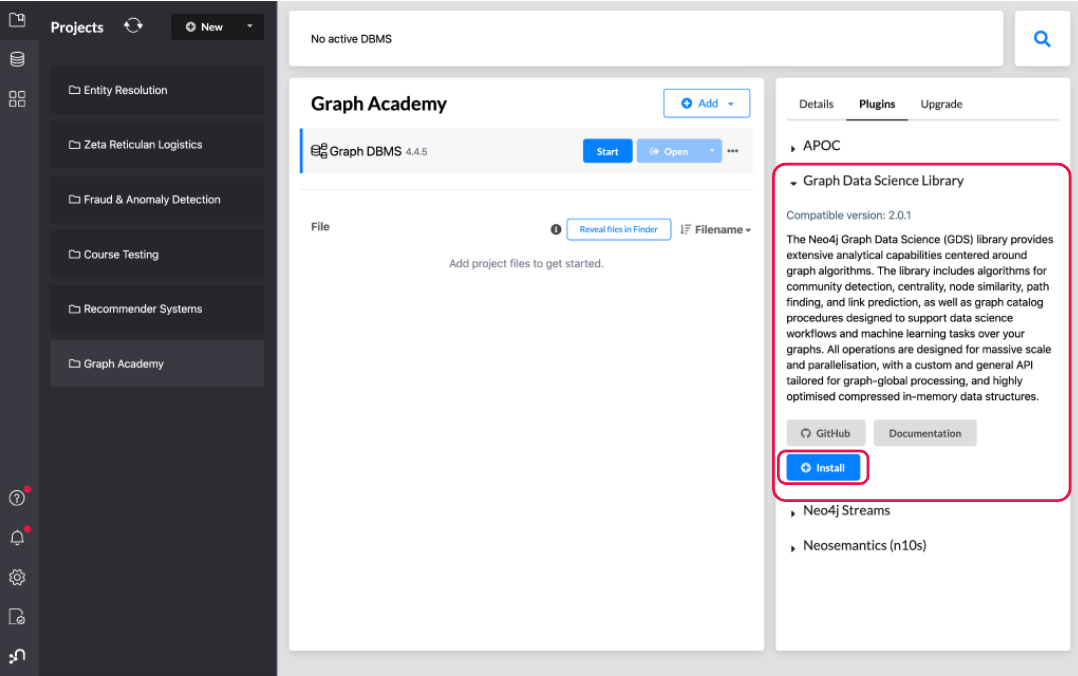
\includegraphics[width=0.7\linewidth,keepaspectratio]{neo4j93}
\end{center}	

{\tiny (Ref: Introduction to Neo4j Graph Data Science - neo4j)}
\end{frame}

%%%%%%%%%%%%%%%%%%%%%%%%%%%%%%%%%%%%%%%%%%%%%%%%%%%%%%%%%%%%%%%%%%%%%%%%%%%%%%%%%%
\begin{frame}[fragile]\frametitle{How GDS Works}

\begin{itemize}
\item At a high-level, GDS works by transforming and loading data into an in-memory format that is optimized for high-performance graph analytics. 
\item GDS provides graph algorithms, feature engineering, and machine learning methods to execute on this in-memory graph format.
\item Workflow: 
	\begin{itemize}
	\item Read data from the Neo4j database, transform it, and load it into an in-memory graph (aka  projecting a graph and refer to the in-memory graph as a graph projection). Collection of graph projections is called as Graph Catalog
	\item Execute Algorithms
	\item Store Results
	\end{itemize}
\end{itemize}

\begin{center}
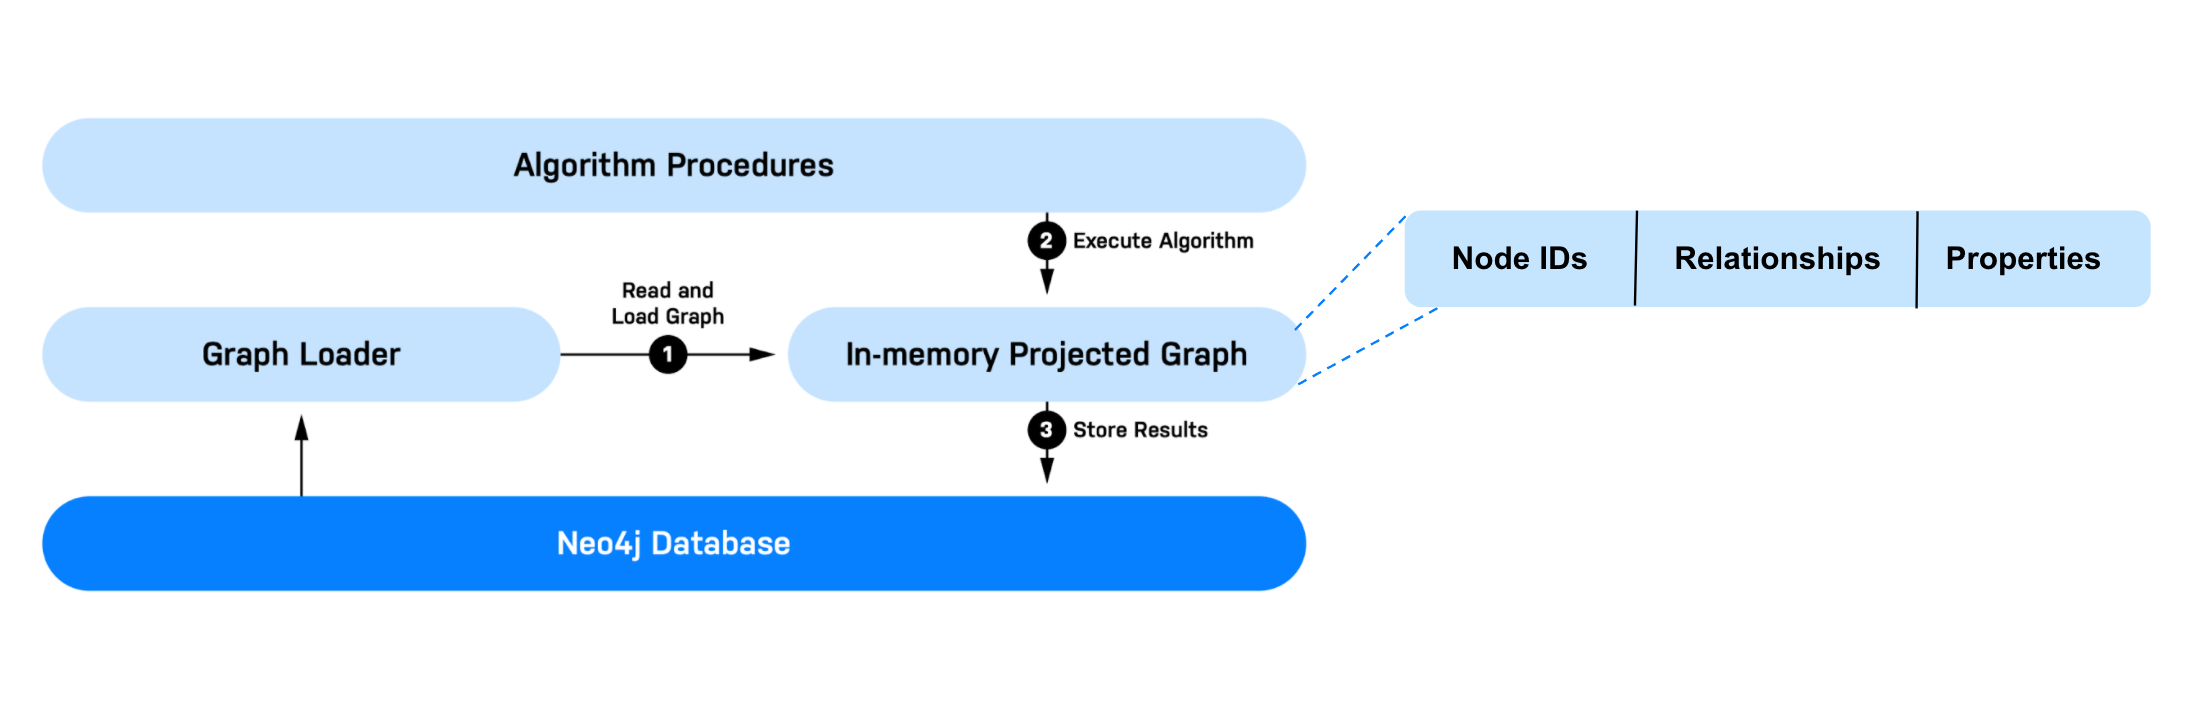
\includegraphics[width=0.8\linewidth,keepaspectratio]{neo4j94}
\end{center}	

{\tiny (Ref: Introduction to Neo4j Graph Data Science - neo4j)}
\end{frame}

%%%%%%%%%%%%%%%%%%%%%%%%%%%%%%%%%%%%%%%%%%%%%%%%%%%%%%%%%%%%%%%%%%%%%%%%%%%%%%%%%%
\begin{frame}[fragile]\frametitle{GDS Configuration}
\begin{columns}
\begin{column}{0.5\textwidth}

\begin{itemize}
\item GDS runs greedily in respect to system resources which means it will use as much memory and CPU cores as it needs - not exceeding limits configured by the user.
\item GDS uses multiple CPU cores for graph projections, algorithms, and writing results. This allows GDS to parallelize its computations and significantly speed up processing time.
\item GDS runs within a Neo4j instance and is therefore subject to the general Neo4j memory configuration. 
\end{itemize}

\end{column}
\begin{column}{0.5\textwidth}  %%<--- here

\begin{center}
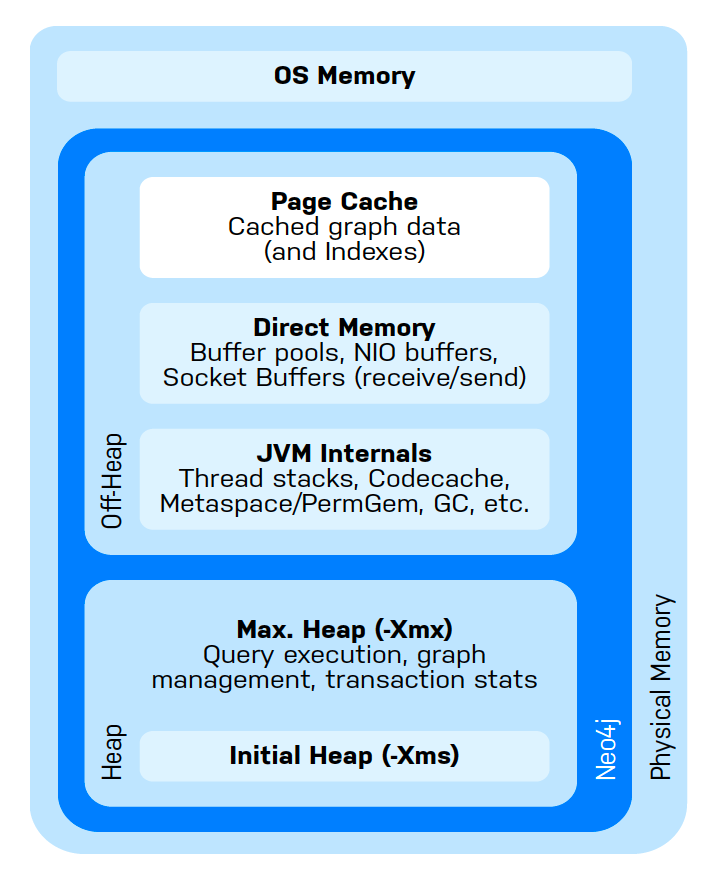
\includegraphics[width=0.8\linewidth,keepaspectratio]{neo4j95}
\end{center}	

{\tiny (Ref: Introduction to Neo4j Graph Data Science - neo4j)}
\end{column}
\end{columns}
\end{frame}

%%%%%%%%%%%%%%%%%%%%%%%%%%%%%%%%%%%%%%%%%%%%%%%%%%%%%%%%%%%%%%%%%%%%%%%%%%%%%%%%%%
\begin{frame}[fragile]\frametitle{Graph Catalog}

\begin{itemize}
\item You can call graph catalog operations with commands of the form \lstinline|CALL gds.graph.<command>|
\item For example, we can list the graph projections that currently exist in our database with  \lstinline|CALL gds.graph.list()|
\item In the recommendations graph, we can create a projection from the Actor and Movie nodes and the ACTED\_IN relationship with \lstinline|CALL gds.graph.project('my-graph-projection', ['Actor','Movie'], 'ACTED_IN')|
\item Now list graphs again we should see information on the graph we just made \lstinline|CALL gds.graph.list() YIELD graphName, nodeCount, relationshipCount, schema|
\end{itemize}

\begin{center}
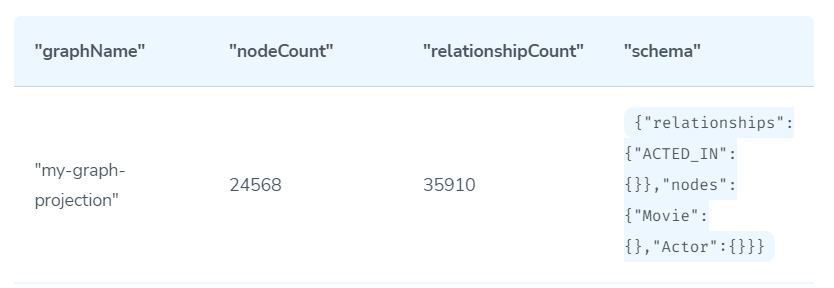
\includegraphics[width=0.8\linewidth,keepaspectratio]{neo4j96}
\end{center}	

{\tiny (Ref: Introduction to Neo4j Graph Data Science - neo4j)}
\end{frame}

%%%%%%%%%%%%%%%%%%%%%%%%%%%%%%%%%%%%%%%%%%%%%%%%%%%%%%%%%%%%%%%%%%%%%%%%%%%%%%%%%%
\begin{frame}[fragile]\frametitle{Running Algorithms}

\begin{itemize}
\item Say, run degree centrality on Actor nodes. 
\item \lstinline|CALL gds.degree.mutate('my-graph-projection', {mutateProperty:'numberOfMoviesActedIn'})|
\item This will count the number of movies each actor was in and store it on a node property called numberOfMoviesActedIn inside the projection (it will not be written back to the database yet).
\item The graph catalog has two methods for export:
\begin{itemize}
\item gds.graph.export to export a graph into a new database - effectively copying the projection into a separate Neo4j database
\item 
gds.beta.graph.export.csv to export a graph to csv files
\end{itemize}

\item  To write the property back to the database we could use the writeNodeProperties operation: \lstinline|CALL gds.graph.writeNodeProperties('my-graph-projection',['numberOfMoviesActedIn'], ['Actor'])|
\item To take the results from our algorithm calculations and stream them into another process:
\end{itemize}

\begin{lstlisting}
CALL gds.graph.streamNodeProperty('my-graph-projection','numberOfMoviesActedIn')
YIELD nodeId, propertyValue
RETURN gds.util.asNode(nodeId).name AS actorName, propertyValue AS numberOfMoviesActedIn
ORDER BY numberOfMoviesActedIn DESCENDING, actorName LIMIT 10| 
\end{lstlisting}

\end{frame}

%%%%%%%%%%%%%%%%%%%%%%%%%%%%%%%%%%%%%%%%%%%%%%%%%%%%%%%%%%%%%%%%%%%%%%%%%%%%%%%%%%
\begin{frame}[fragile]\frametitle{Projects}

There are 2 primary types of projections in GDS, native projections and cypher projections.

\begin{itemize}
\item Native projections are optimized for efficiency and performance to support graph data science at scale.
\item Cypher projections are optimized for flexibility and customization to support exploratory analysis, experimentation, and smaller graph projections.
\item  When you call \lstinline|gds.graph.project()| you are using a native projection. 
\item Native projections provide the best performance by reading from the Neo4j store files directly
\item Additional features:
	\begin{itemize}
	\item the inclusion of numeric node and relationship properties
	\item altering relationship direction or "orientation"
		\begin{itemize}
			\item NATURAL: same direction as in the database (default)
			\item REVERSE: opposite direction as in the database
			\item UNDIRECTED: undirected
			\end{itemize}

	\item aggregating parallel relationships
	\end{itemize}
\item If you attempt to create a new graph projection with a name that already exists, you will receive an error. To continue you will first have to run the gds.graph.drop() procedure to drop the existing graph projection.
\item '*' can be used to include all nodes and/or relationships in the database.
\end{itemize}

\end{frame}

%%%%%%%%%%%%%%%%%%%%%%%%%%%%%%%%%%%%%%%%%%%%%%%%%%%%%%%%%%%%%%%%%%%%%%%%%%%%%%%%%%
\begin{frame}[fragile]\frametitle{Including Node and Relationship Properties}

There are 2 primary types of projections in GDS, native projections and cypher projections.

\begin{itemize}
\item Node and relationship properties may be useful to consider in graph analytics. 
\item They can be used as weights in graph algorithms and features for machine learning.
\item Below is an example of including multiple movie node properties and the rating relationship property.
\end{itemize}

\begin{lstlisting}
CALL gds.graph.drop('native-proj', false);

CALL gds.graph.project(
    'native-proj',
    ['User', 'Movie'],
    {RATED: {orientation: 'UNDIRECTED'}},
    {
        nodeProperties:{
            revenue: {defaultValue: 0}, // (1)
            budget: {defaultValue: 0},
            runtime: {defaultValue: 0}
        },
        relationshipProperties: ['rating'] // (3)
    }
);
\end{lstlisting}

\end{frame}

%%%%%%%%%%%%%%%%%%%%%%%%%%%%%%%%%%%%%%%%%%%%%%%%%%%%%%%%%%%%%%%%%%%%%%%%%%%%%%%%%%
\begin{frame}[fragile]\frametitle{Parallel Relationship}

\begin{itemize}
\item The Neo4j database allows you to store multiple relationships of the same type and direction between two nodes.
\item These are colloquially known as parallel relationships. 
\item For example, consider a graph of financial transaction data where users send money to one another. If a user sends money to the same user multiple times this can form multiple parallel relationships.
\end{itemize}

\begin{center}
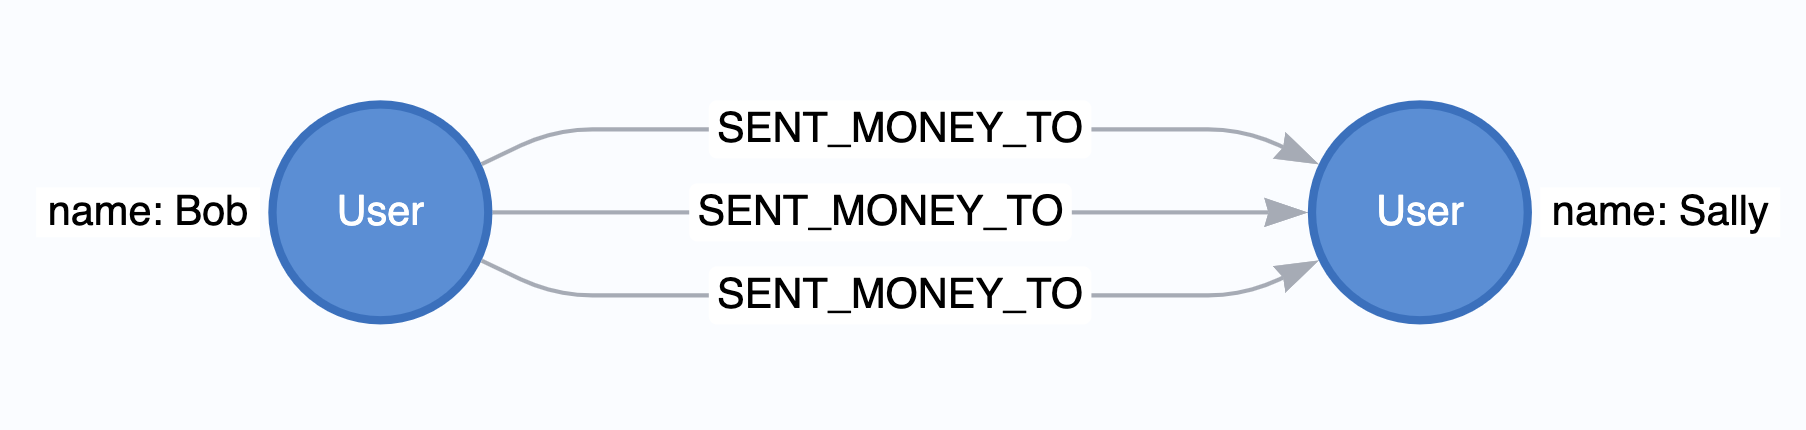
\includegraphics[width=0.8\linewidth,keepaspectratio]{neo4j97}
\end{center}	

{\tiny (Ref: Introduction to Neo4j Graph Data Science - neo4j)}
\end{frame}

%%%%%%%%%%%%%%%%%%%%%%%%%%%%%%%%%%%%%%%%%%%%%%%%%%%%%%%%%%%%%%%%%%%%%%%%%%%%%%%%%%
\begin{frame}[fragile]\frametitle{Parallel Relationship Aggregation}

\begin{itemize}
\item Sometimes you will want to aggregate these parallel relationships into a single relationship in preparation for running graph algorithms or machine learning. 
\item This is because graph algorithms may count each relationship between two nodes separately when all we need to consider is whether a single relationship exists between them. 
\item Other times we may want to weight the connection between two nodes higher if more parallel relationships exists, but it’s not always easy to do so without aggregating the relationships first depending on which algorithm you use.
\end{itemize}

\begin{center}
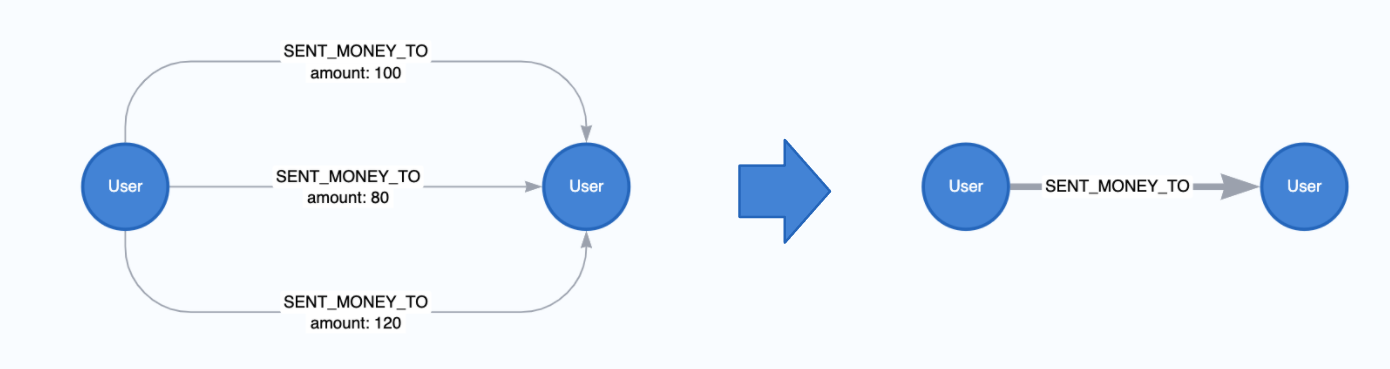
\includegraphics[width=0.8\linewidth,keepaspectratio]{neo4j98}
\end{center}	

{\tiny (Ref: Introduction to Neo4j Graph Data Science - neo4j)}

\begin{lstlisting}
CALL gds.graph.project(
  'user-proj',
  ['User'],
  {
    SENT_MONEY_TO: { aggregation: 'SINGLE' }
  }
);
\end{lstlisting}
\end{frame}

%%%%%%%%%%%%%%%%%%%%%%%%%%%%%%%%%%%%%%%%%%%%%%%%%%%%%%%%%%%%%%%%%%%%%%%%%%%%%%%%%%
\begin{frame}[fragile]\frametitle{Parallel Relationship Aggregation}

We can create a property with the count of the relationships as well - like so:

\begin{center}
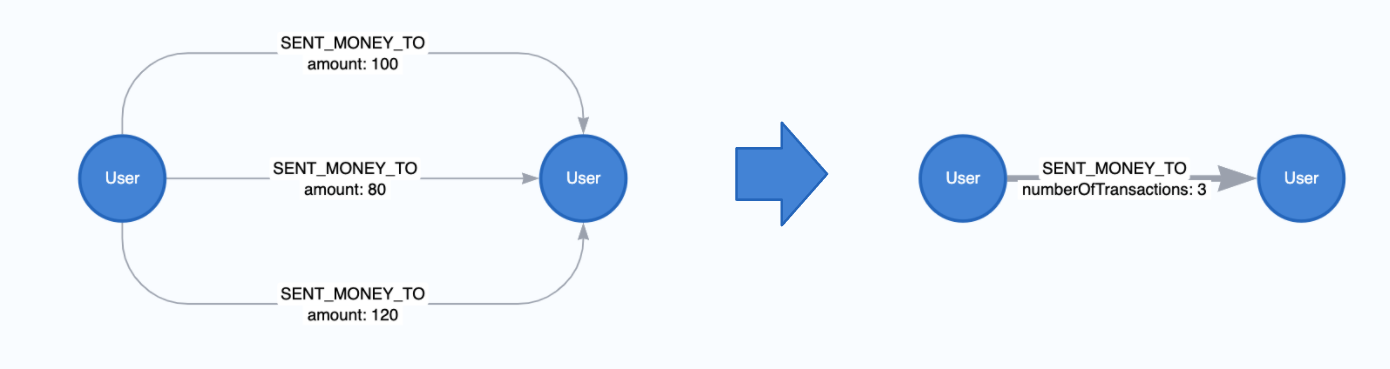
\includegraphics[width=0.8\linewidth,keepaspectratio]{neo4j99}
\end{center}	

{\tiny (Ref: Introduction to Neo4j Graph Data Science - neo4j)}

\begin{lstlisting}
CALL gds.graph.project(
  'user-proj',
  ['User'],
  {
    SENT_MONEY_TO: {
      properties: {
        numberOfTransactions: {
          // the wildcard '*' is a placeholder, signaling that
          // the value of the relationship property is derived
          // and not based on Neo4j property.
          property: '*',
          aggregation: 'COUNT'
        }
      }
    }
  }
);
\end{lstlisting}
\end{frame}

